\documentclass[9pt]{article}

\usepackage{amssymb}
\usepackage{amsmath}
\usepackage{amsfonts}
\usepackage{comment}
\usepackage{fancyhdr}
\usepackage{mathrsfs}
\usepackage{enumitem}
\usepackage{graphicx}

\usepackage{tikz}

\voffset = -50pt
%\textheight = 700pt
\addtolength{\textwidth}{60pt}
\addtolength{\evensidemargin}{-30pt}
\addtolength{\oddsidemargin}{-30pt}
%\setlength{\headheight}{44pt}

\newcommand{\qed}{\hfill \ensuremath{\Box}}


\newcommand*\circled[1]{\tikz[baseline=(char.base)]{
            \node[shape=circle,draw,inner sep=2pt] (char) {#1};}}

\newcommand{\Z}{\mathbb{Z}}
\newcommand{\I}{\mathbb{I}}
\newcommand{\M}{\mathbb{M}}
\newcommand{\R}{\mathbb{R}}
\newcommand{\C}{\mathbb{C}}
%\setcounter{section}{-1}

\begin{document}
\topskip0pt
\vspace*{\fill}
\begin{center}
{\Huge \begin{tabular}{@{}ll@{}}
   Class: & CECS 201, Section 7 \\ \\ \\
   Lab: & 8 \\ \\ \\
   Title: & Latches and Flip-Flops \\ \\ \\
   Student Name: & Barry Joseph Okonoboh \\ \\ \\
   Due Date: & 11:59:59 P.M., 13, April 2015 \\ \\ \\
   Instructor: & Dan Cregg
\end{tabular}}
\end{center}
\vspace*{\fill}
\newpage
\begin{enumerate}
%%%%%%%%%%%%%%%%%%%%%%%%%%%%%%%%%%%%%%%%01%%%%%%%%%%%%%%%%%%%%%%%%%%%%%%%%%%%%%%
   \item[\textbf{Introduction.}]  We investigate the functions of an S-R Latch,
             a D Flip-Flop, a T Flip-flop and a J-K Flip-Flip, and the
             differences between them.
   \item[\textbf{Project Description.}] \textbf{S-R Latch's Truth Table}
         \begin{center}
    \begin{tabular}{@{}|c|c|c|@{}}
   \hline
         S & R & $Q_1$ \\ \hline
         0 & 0 & $Q_1$ \\ \hline
         0 & 1 & 0 \\ \hline
         1 & 0 & 1 \\ \hline
         1 & 1 & ?? \\ \hline         
\end{tabular}
   \end{center}
   
         For the S-R latch, we notice that if the clock rises from 0 to 1, then
         \begin{itemize}
            \item $Q_1$ will be set to 1 if $S = 1$ and $R = 0$.
            \item $Q_1$ will be set to 0 if $S = 0$ and $R = 1$.
            \item $Q_1$'s state will be unchanged if $S = R = 0$.
            \item indeterminate if $S = R = 1$.            
         \end{itemize}
         
         Also the state of $Q_1$ does not change if the clock is not set. \\
         
          \textbf{D Flip-Flop's Truth Table}
         \begin{center}
    \begin{tabular}{@{}|c|c|@{}}
   \hline
         D & $Q$  \\ \hline
         0 & 0  \\ \hline
         1 & 1  \\ \hline       
\end{tabular}
   \end{center}
   
      On a positive clock edge, $Q$ will attain the value of input D. If the
      clock is not set, then varying the input D will have no effect on $Q$, as
      evidenced in the lab. \\ \\
         
         \textbf{T Flip-Flop's Truth Table}
         \begin{center}
    \begin{tabular}{@{}|c|c|c|c|@{}}
   \hline
         T & $Q$ & $Q_{next}$ & Operation  \\ \hline
         0 & 0 & 0 & Hold \\ \hline
         0 & 1 & 1 & Hold \\ \hline
         1 & 0 & 1 & Toggle \\ \hline
         1 & 1 & 0 & Toggle \\ \hline       
\end{tabular}
   \end{center}
   
      The T Flip-Flops stores the value of its output if T is 0. But if T is 1,
      it negates the value in $Q$. The $Q_{next}$ columns holds the future
      value of $Q$ on a positive clock edge. \\ \\
      
      \textbf{J-K Flip-Flop's Truth Table}
         \begin{center}
    \begin{tabular}{@{}|c|c|c|c|c|@{}}
   \hline
         J & K & $Q$ & $Q_{next}$ & Operation  \\ \hline
         0 & 0 & 0 & 0 & Hold \\ \hline
         0 & 0 & 1 & 1 & Hold \\ \hline
         0 & 1 & 0 & 0 & Reset \\ \hline
         0 & 1 & 1 & 0 & Reset \\ \hline
         1 & 0 & 0 & 1 & Set \\ \hline  
         1 & 0 & 1 & 1 & Set \\ \hline
         1 & 1 & 0 & 1 & Toggle \\ \hline
         1 & 1 & 1 & 0 & Toggle \\ \hline           
\end{tabular}
   \end{center}
   
      As the lab and Truth Table showed us, a J-K Flip-Flop is a combination of a
      D Flip-Flop and a T-Flip Flop. We can select particular values for J and K
      so that it can mimic the behavior of a D Flip-Flop or a T-Flip Flop.
      

  	\item[\textbf{Schematic.}] \text{ }
   
             \begin{center}
                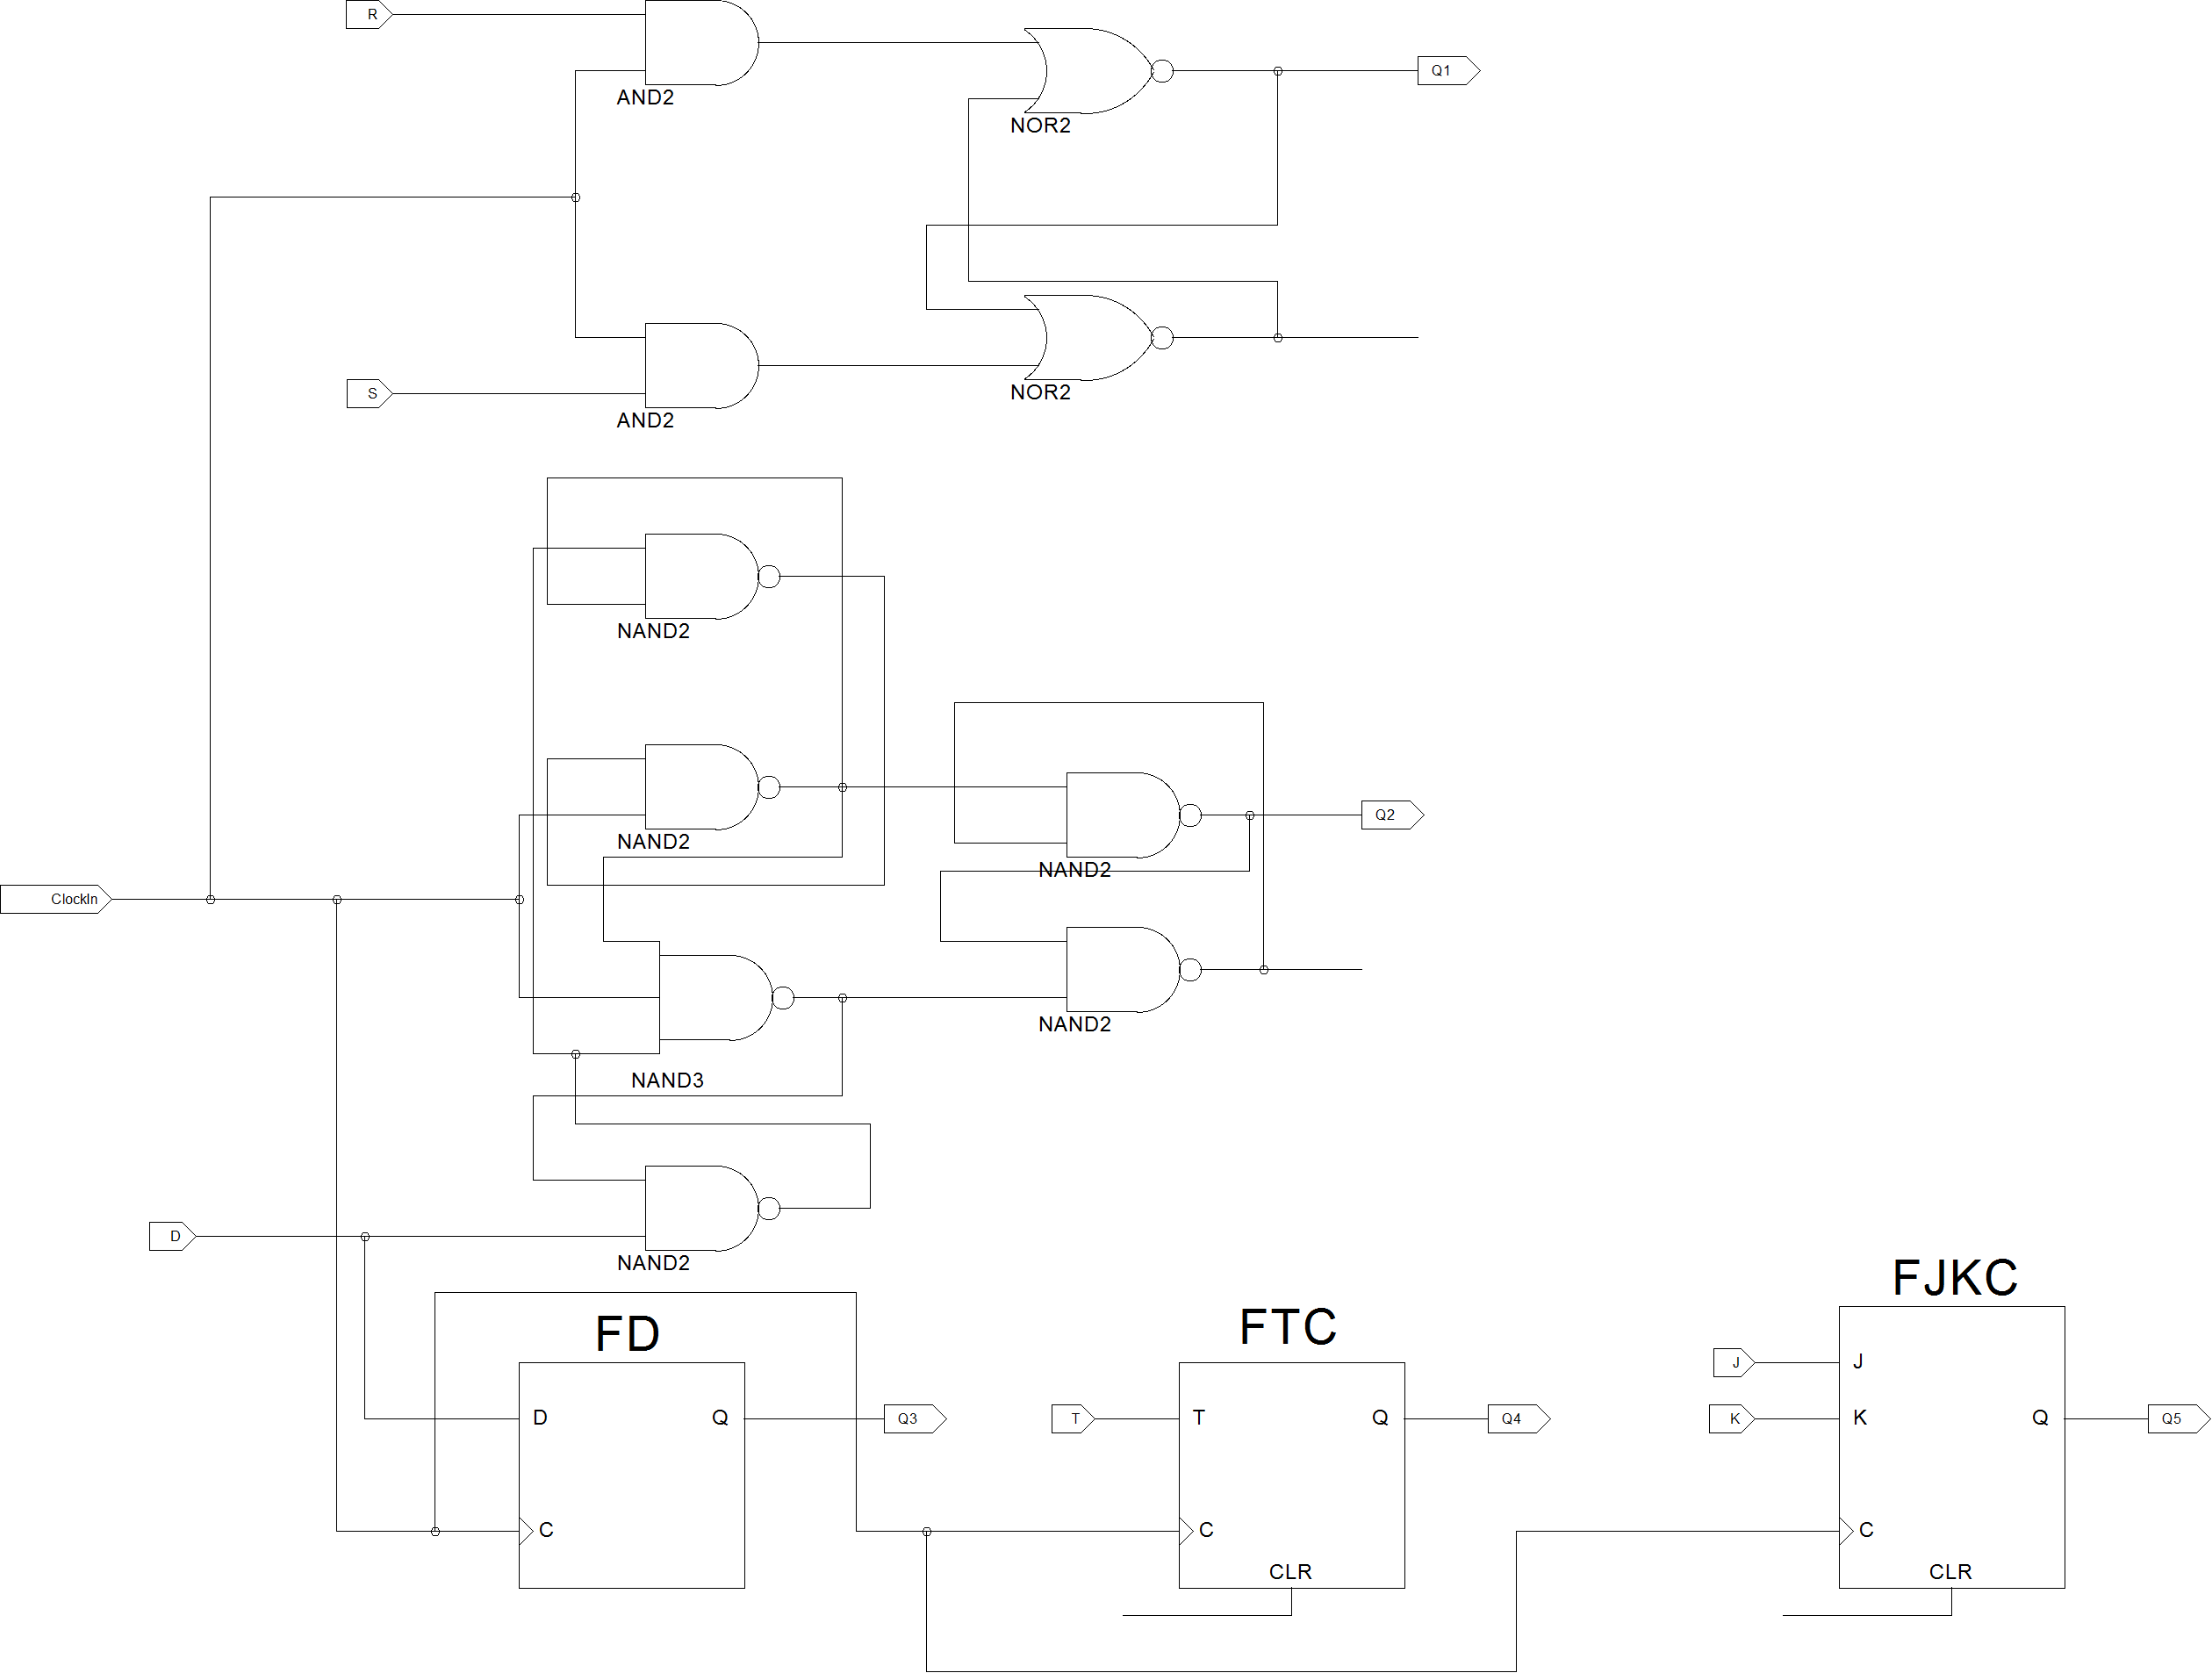
\includegraphics[width=\textwidth]{schematic.png}
             \end{center} 
   
   
\end{enumerate}
\end{document}
